\documentclass{beamer}
%
% Choose how your presentation looks.
%
% For more themes, color themes and font themes, see:
% http://deic.uab.es/~iblanes/beamer_gallery/index_by_theme.html
%

\mode<presentation>
{
  \usetheme{Darmstadt}      % or try Darmstadt, Madrid, Warsaw, ...
  \usecolortheme{default} % or try albatross, beaver, crane, ...
  \usefonttheme{default}  % or try serif, structurebold, ...
  \setbeamertemplate{navigation symbols}{}
  \setbeamertemplate{caption}[numbered]
} 
\setbeamertemplate{footline}{%
    \hspace{0.94\paperwidth}%
    \usebeamerfont{title in head/foot}%
    \insertframenumber\,/\,\inserttotalframenumber%
}
\usepackage[T2A]{fontenc}
\usepackage[russian, english]{babel}
\usepackage[utf8]{inputenc}
%\usepackage{pagenumber}
%\pagestyle{plain}
\title[Nvidia CUDA и AMD FireStream]{Сравнение Nvidia CUDA и AMD FireStream}
\author{Аметов И.И.}
\institute{Московский Технологический институт}
\date{19.11.2017}

\begin{document}
\def\figurename{Рисунок}
\def\tablename{Таблица}
\begin{frame}
  \titlepage
\end{frame}

% Uncomment these lines for an automatically generated outline.
%\begin{frame}{Outline}
%  \tableofcontents
%\end{frame}

\section{История развития видеокарт}

\begin{frame}{MDA (Monochrome Display Adapter)}

\begin{figure}
\center
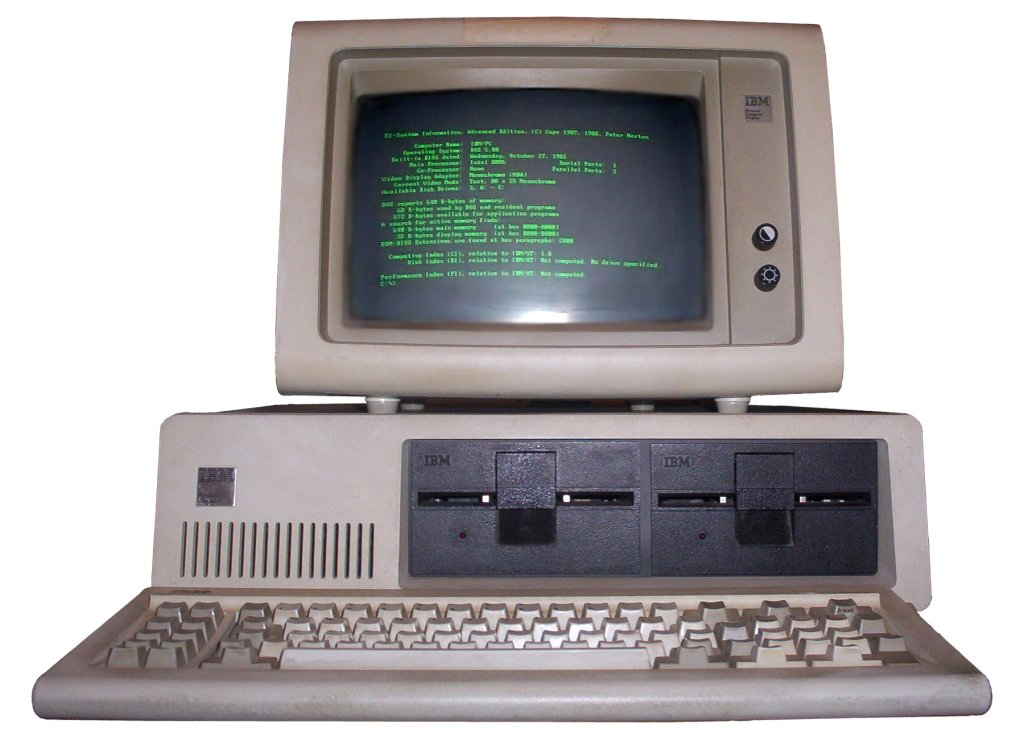
\includegraphics[width=0.5\textwidth]{Images/IBM_PC_5150.jpg}
\caption{\label{fig:MDA}<<Зелёный>> монохромный монитор для MDA.}
\end{figure}

\begin{itemize}
  \item{ Год выпуска: 1981.}
  \item{Производитель: IBM.}
  \item{Поддерживаемые режимы: текстовый --- $80 \times 25$ символов.}
\end{itemize}

%\vskip 1cm

%\begin{block}{Examples}
%Some examples of commonly used commands and features are included, to help you get started.
%\end{block}

\end{frame}

\begin{frame}{HGC (Hercules Graphics Controller)}

\begin{figure}
\center
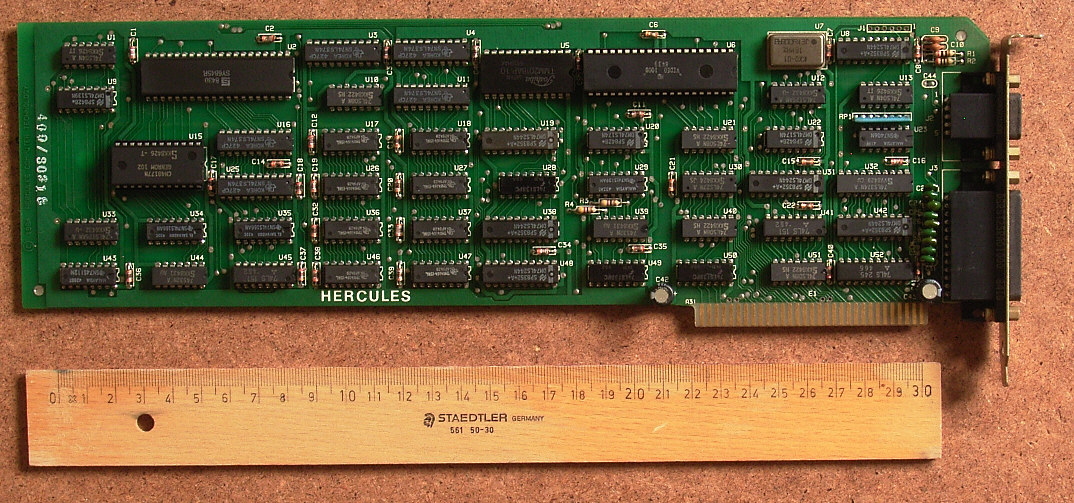
\includegraphics[width=0.5\textwidth]{Images/Hercules_Graphics_Card.jpg}
\caption{\label{fig:HGC}Видеоадаптер Hercules Graphics Controller.}
\end{figure}

\begin{itemize}
\item{Год выпуска: 1982.}
\item{Производитель: Hercules Computer Technology.}
\item{Поддерживаемые режимы: графическое разрешение $720 \times 348$ точек.}
\end{itemize}

\end{frame}

\begin{frame}{CGA (Color Graphics Adapter)}

\begin{figure}
\center
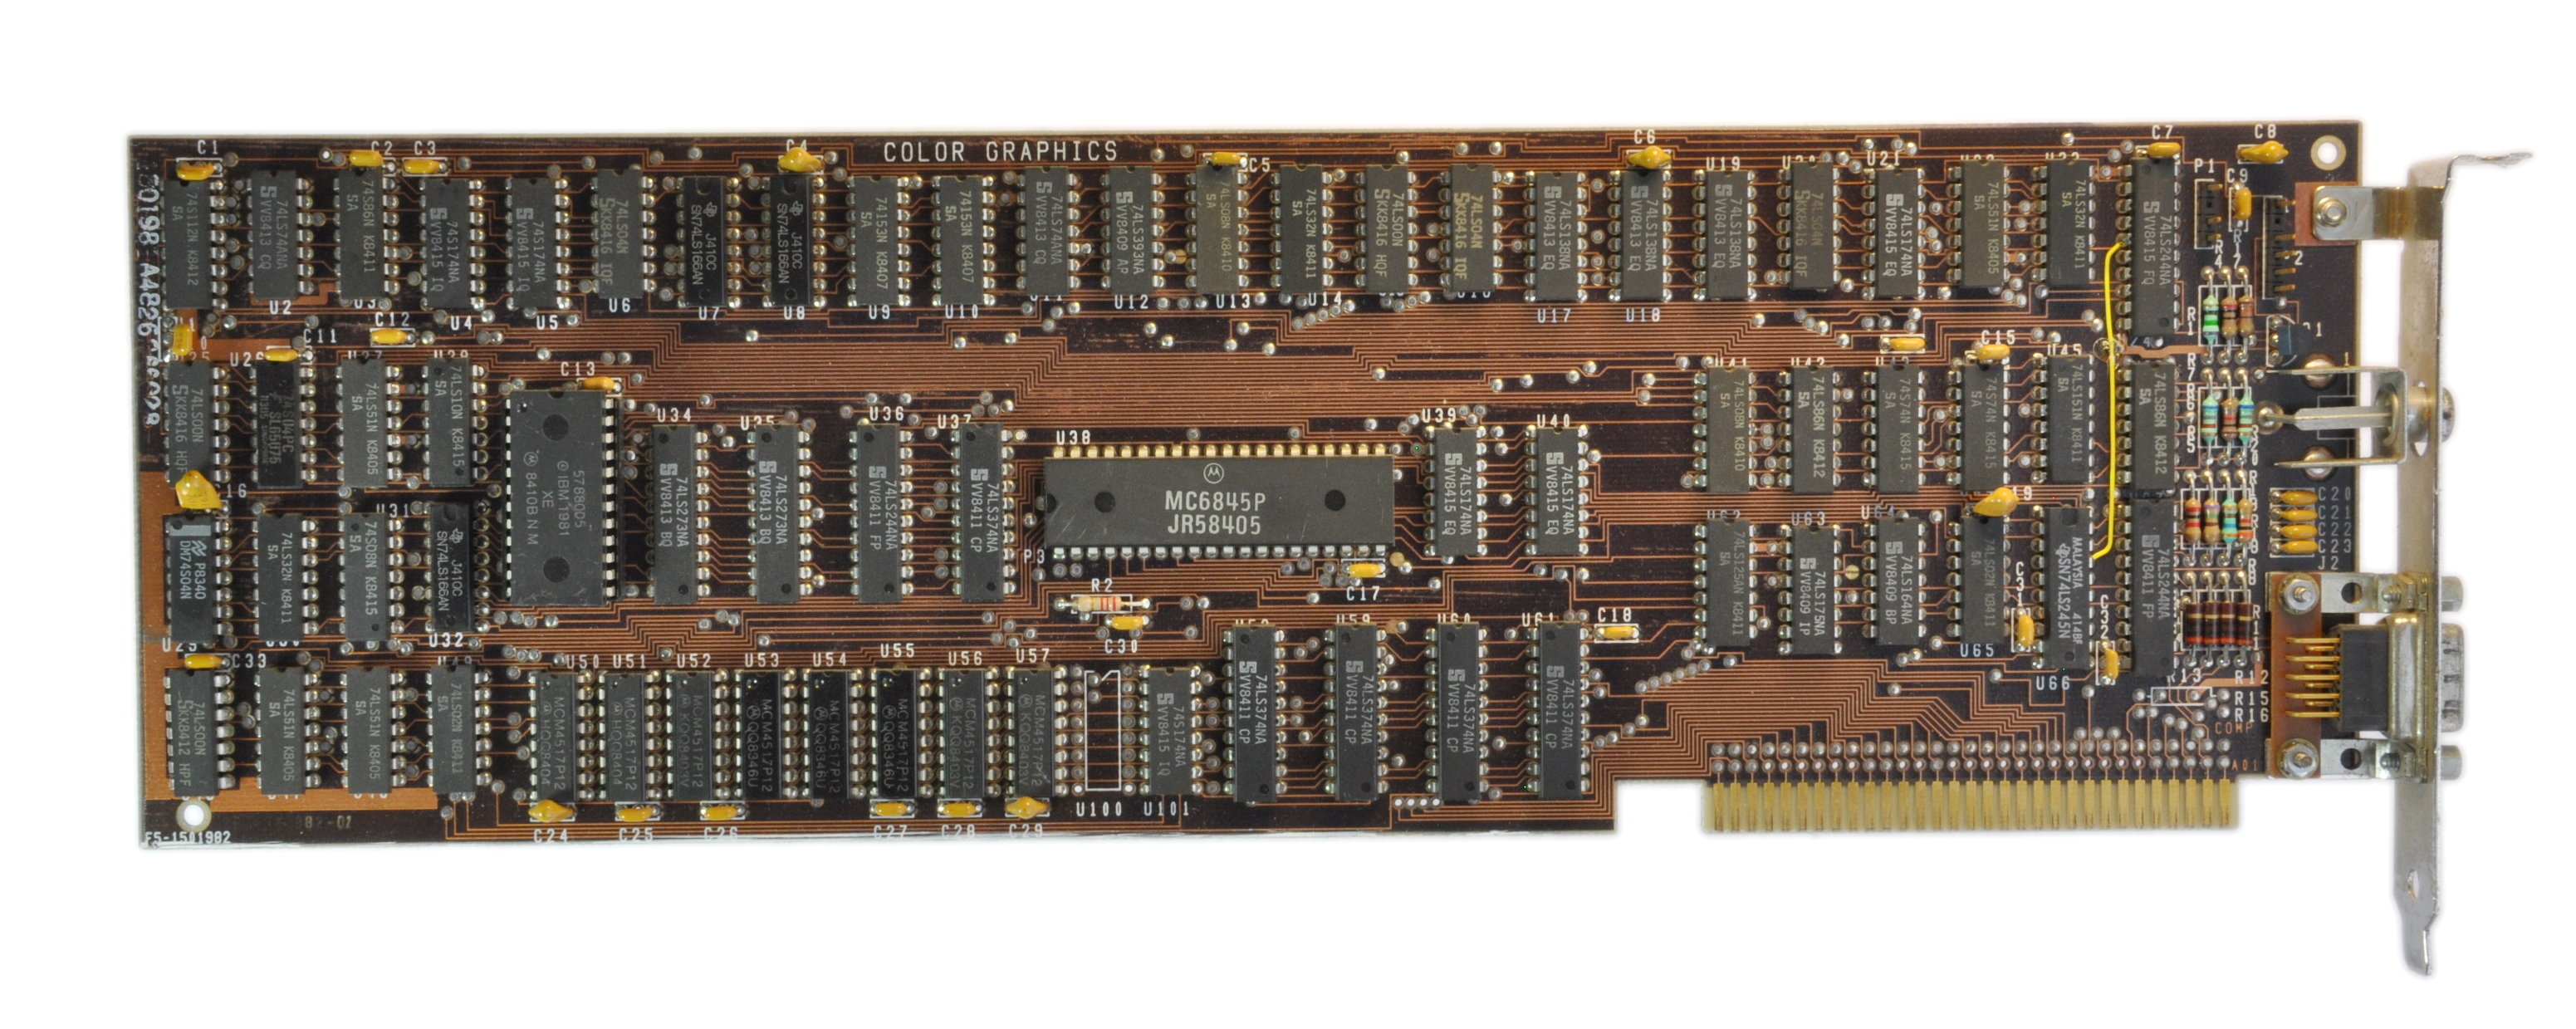
\includegraphics[width=0.5\textwidth]{Images/IBM_Color_Graphics_Adapter.jpg}
\caption{\label{fig:CGA}Видекарта Color Graphics Adapter.}
\end{figure}

\begin{itemize}
\item{Год выпуска: 1981.}
\item{Производитель: IBM.}
\item{Поддерживаемые режимы: }

\begin{itemize}
\item{текстовый --- $40 \times 25$ и $80 \times 25$ символов 16 цветов символа и 16 цветов фона}
\item{графический --- $320 \times 200$ (четыре палитры по четыре цвета) и $640 \times 200$ (монохромный)}
\end{itemize}

\end{itemize}

\end{frame}

\begin{frame}{EGA (Enhanced Graphics Adapter)}

\begin{figure}
\center
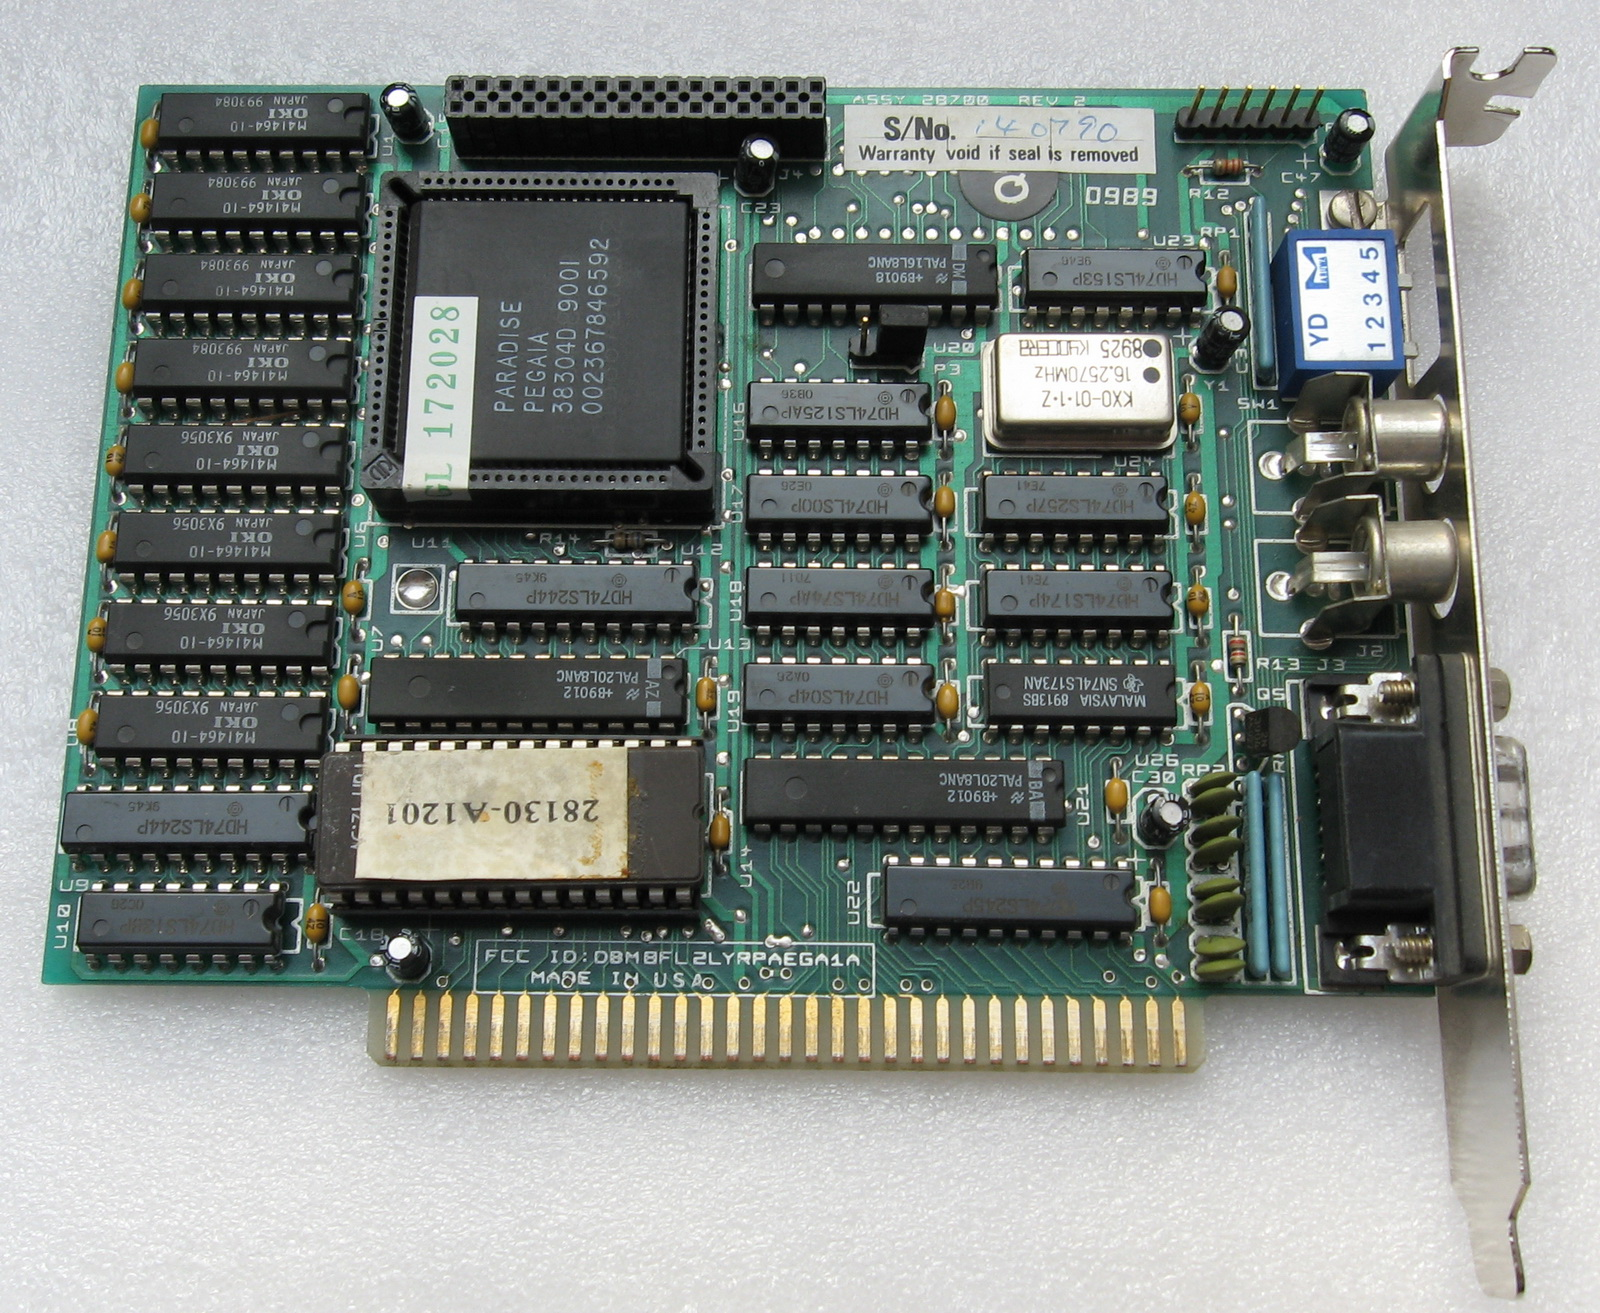
\includegraphics[width=0.5\textwidth]{Images/EGA_card.jpg}
\caption{\label{fig:EGA}Видекарта Enhanced Graphics Adapter.}
\end{figure}

\begin{itemize}
\item{Год выпуска: 1984.}
\item{Производитель: IBM.}
\item{Поддерживаемые режимы: }

\begin{itemize}
\item{графический --- $640 \times 350$ (16 цветов из возможных 64)}
\end{itemize}

\end{itemize}

\end{frame}

\begin{frame}{VGA (Video Graphics Array)}

\begin{figure}
\center
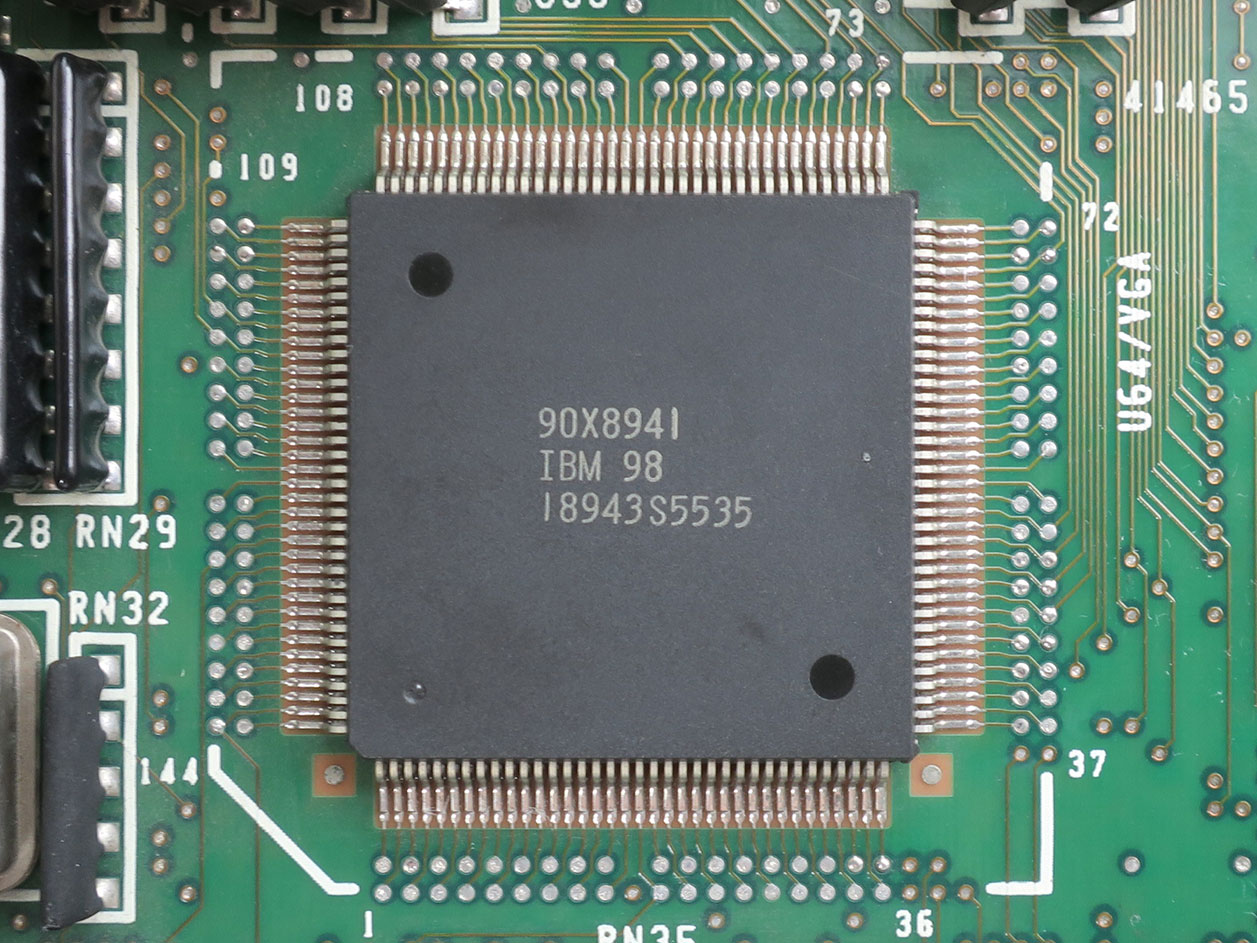
\includegraphics[width=0.5\textwidth]{Images/IBM_VGA.jpg}
\caption{\label{fig:VGA}Видекарта Video Graphics Array.}
\end{figure}

\begin{itemize}
\item{Год выпуска: 1987.}
\item{Производитель: IBM.}
\item{Поддерживаемые режимы: }

\begin{itemize}
\item{графический --- $640 \times 480$ (16 цветов) и $320 \times 200$ (256 цветов)}
\end{itemize}

\end{itemize}

\end{frame}

\section{Устройство современной видеокарты}

\begin{frame}{Устройство современной видеокарты}

\begin{figure}
\center
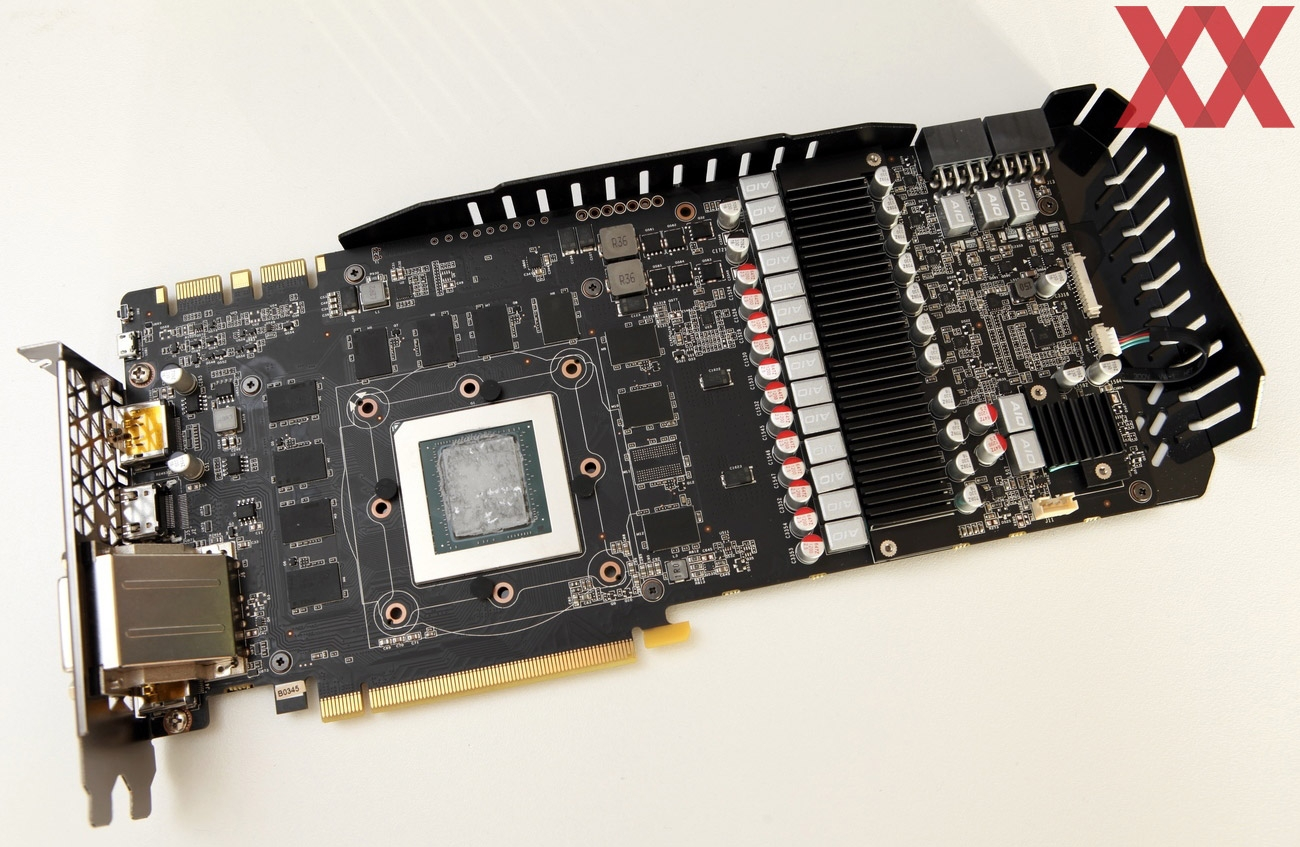
\includegraphics[width=0.6\textwidth]{Images/417-3.jpg}
\caption{\label{fig:GTX1080}Видекарта GeForce GTX 1080 Ti.}
\end{figure}

\end{frame}

\section{Сравнение CPU и GPU}

\begin{frame}{Сравнение CPU и GPU}

\begin{figure}
\center
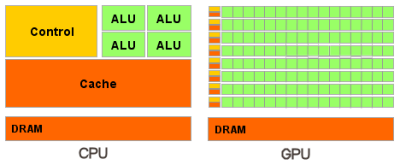
\includegraphics[width=\textwidth]{Images/cpu_vs_gpu.png}
\caption{\label{fig:CPUvsGPU}Сравнение CPU и GPU.}
\end{figure}

\end{frame}

\section{Nvidia CUDA}

\begin{frame}{Nvidia CUDA}

\begin{figure}
\center
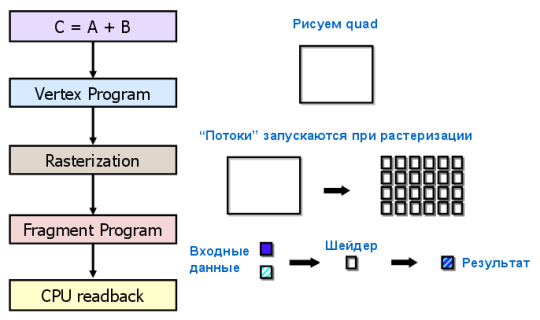
\includegraphics[width=\textwidth]{Images/pipeline2.png}
\caption{\label{fig:pipeline}Процесс работы видеокарты.}
\end{figure}

\end{frame}

\section{AMD FireStream}

\begin{frame}{AMD FireStream}

\begin{table}
\begin{center}
\begin{tabular}{|c|c|c|c|c|}
\hline
\multicolumn{5}{|c|}{Секции инструкций условных переходов} \\
\hline
Секция 0 & Ветвление 0 & \multicolumn{3}{|p{6cm}|}{Ссылка на секцию 3 непрерывных арифметических инструкций} \\ \hline
Секция 1 & Ветвление 1 & \multicolumn{3}{|p{6cm}|}{Ссылка на секцию 4} \\ \hline
Секция 2 & Ветвление 2 & \multicolumn{3}{|p{6cm}|}{Ссылка на секцию 5} \\ \hline
\multicolumn{5}{|c|}{Секции непрерывных арифметических инструкций} \\ \hline
Секция 3 & VLIW 0 & VLIW 1 & VLIW 2 & VLIW 3 \\ \hline
Секция 4 & VLIW 4 & VLIW 5 & & \\ \hline
Секция 5 & VLIW 6 & VLIW 7 & VLIW 8 & VLIW 9 \\ \hline
\end{tabular}
\end{center}
\caption {Схема разбивки программы в архитектуре видеокарт ATI}
\end{table}

\end{frame}

\section{Сравнительная таблица GPU: AMD и Nvidia}

\begin{frame}{Сравнительная таблица GPU: AMD и Nvidia}

\begin{table}
\begin{center}
\begin{tabular}{|p{5cm}|p{5cm}|}
\hline
AMD & Nvidia \\ \hline
Технология FireStream & CUDA \\ \hline
64 нити в блоке & 32 нити в блоке \\ \hline
Использование секций с данными & Традиционное построение программ \\ \hline
Меньше возможности для рекурсии & Больше возможностей для рекурсии \\ \hline
Теоретически более быстрая производительность & Меньшая производительность \\ 
\hline
\end{tabular}

\end{center}
\caption{Краткое сравнение графических процессоров AMD и Nvidia}
\end{table}

\end{frame}

\section{Применение GPU}

\subsection{Медицина}

\begin{frame}{Исследование болезни Паркинсона}

\begin{figure}
\center
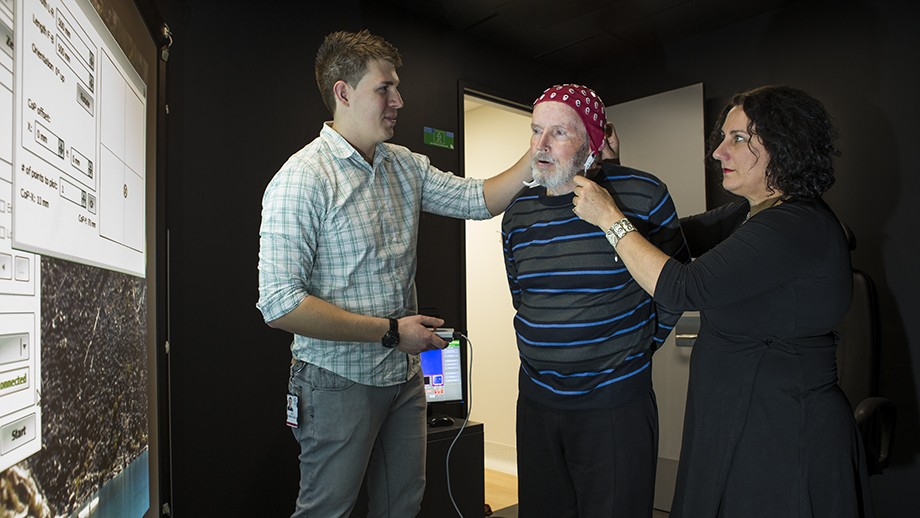
\includegraphics[width=0.7\textwidth]{Images/parkinson.jpg}
\caption{\label{fig:parkinson}Исследователи Алекс Смит (слева) и доктор Дебора Антроп (справа) проводят исследование Кена Худа (в центре), страдающего болезнью Паркинсона. Фотография Стюарта Хэя. Австралийский национальный университет.}
\end{figure}

\end{frame}

\begin{frame}{Zebra Medical Vision}

\begin{figure}
\center
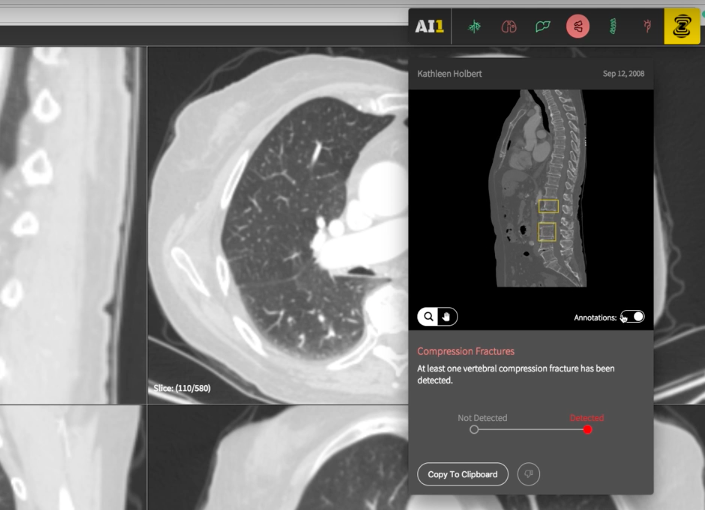
\includegraphics[width=0.7\textwidth]{Images/zebra.png}
\caption{\label{fig:zebra}Искусственный интеллект в радиологии.}
\end{figure}

\end{frame}

\subsection{Энергетика}

\begin{frame}{Солнечная энергия}

\begin{figure}
\center
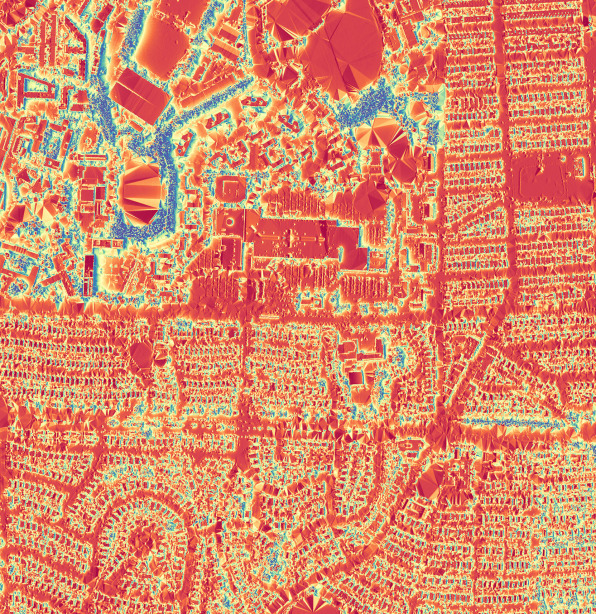
\includegraphics[width=0.5\textwidth]{Images/solar_radiation.jpg}
\caption{\label{fig:solar}Карта солнечного излучения от PowerScout, Калифорния, США.}
\end{figure}

\end{frame}

\subsection{Майнинг криптовалют}

\begin{frame}

\begin{figure}
\center
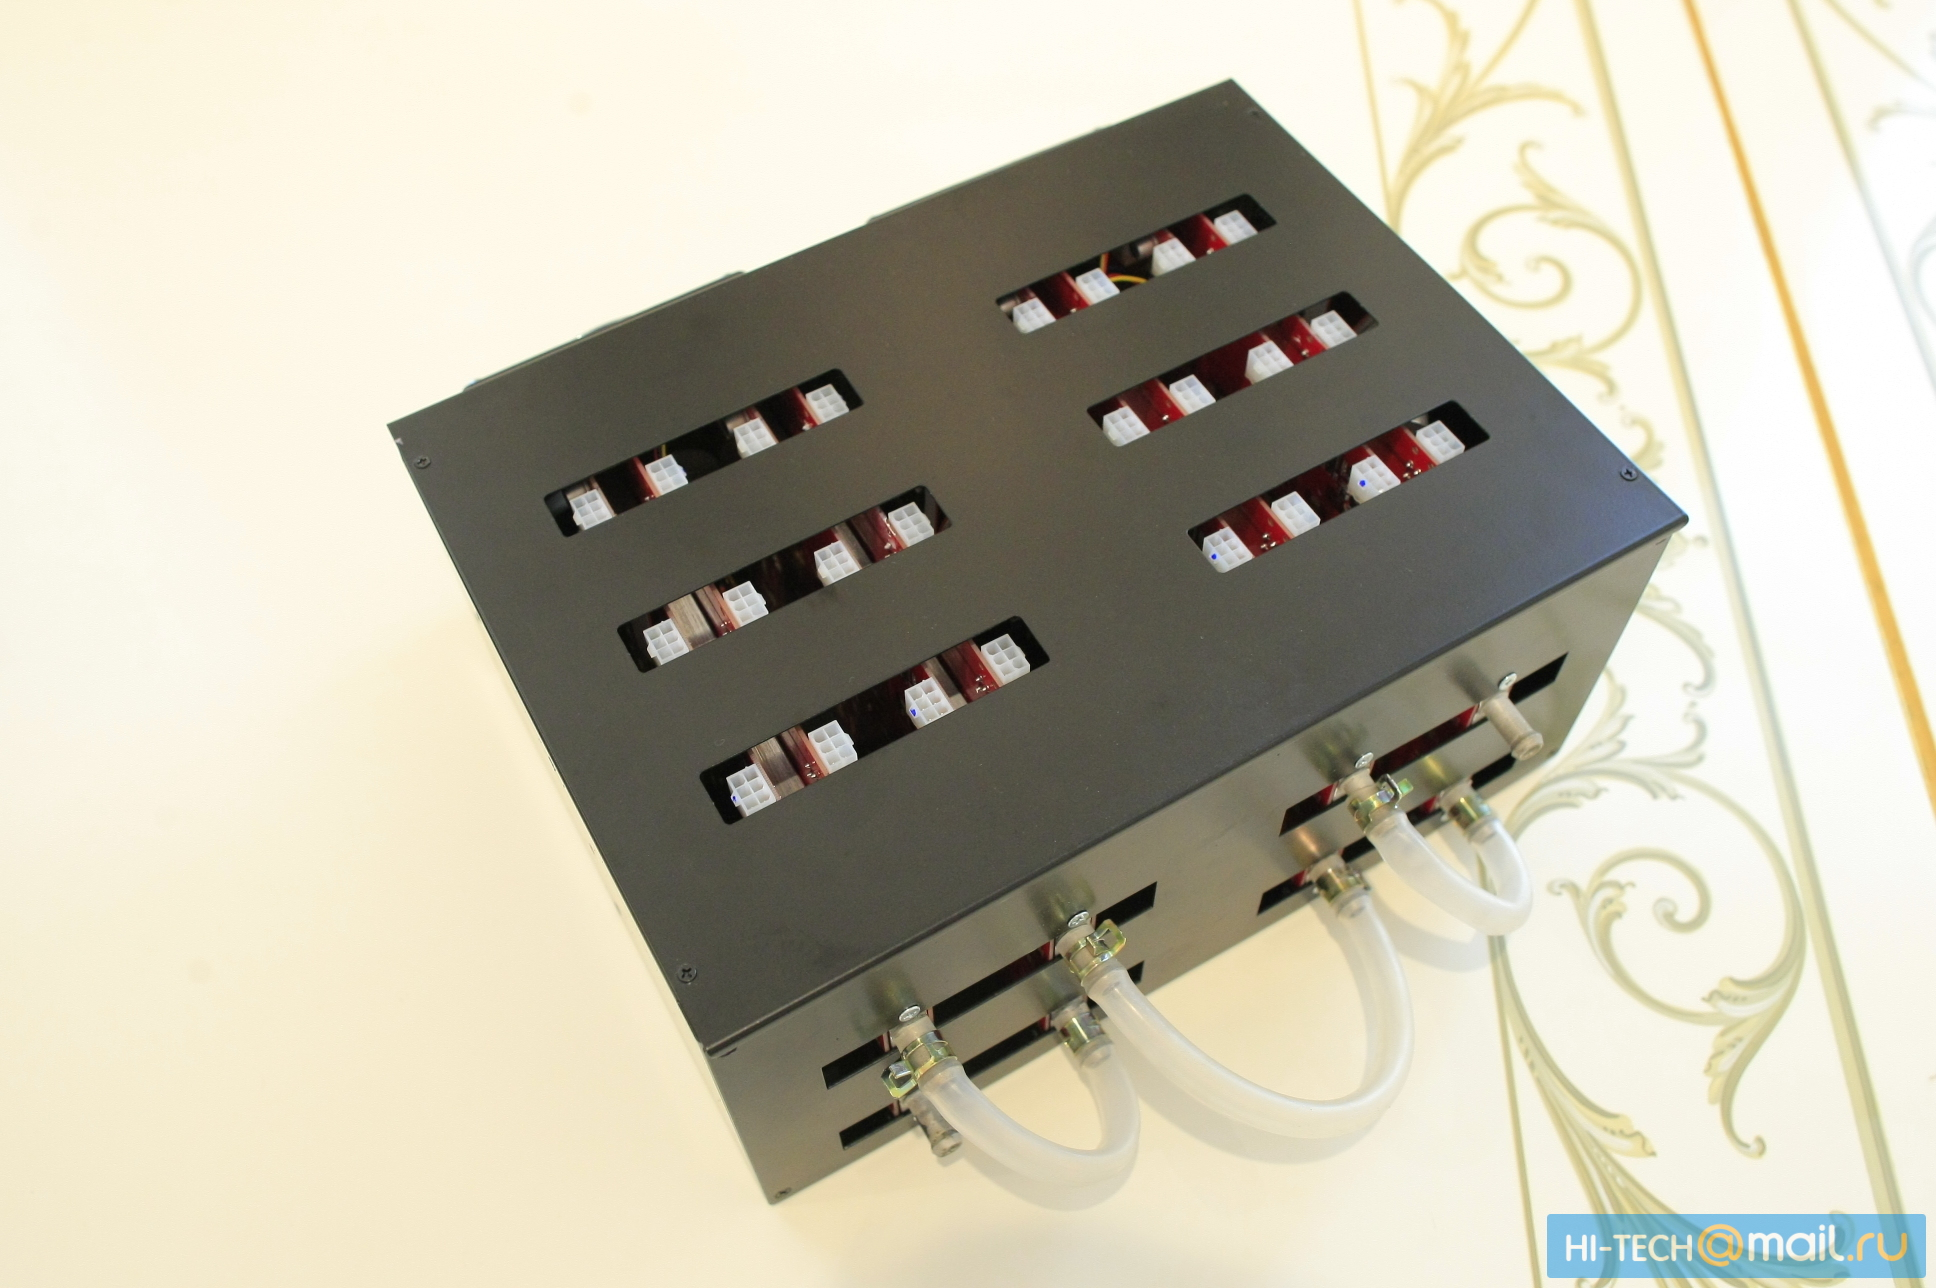
\includegraphics[width=\textwidth]{Images/mining03.jpg}
\caption{\label{fig:mine03}Майнинг-ферма.}
\end{figure}

\end{frame}

\begin{frame}

\begin{figure}
\center
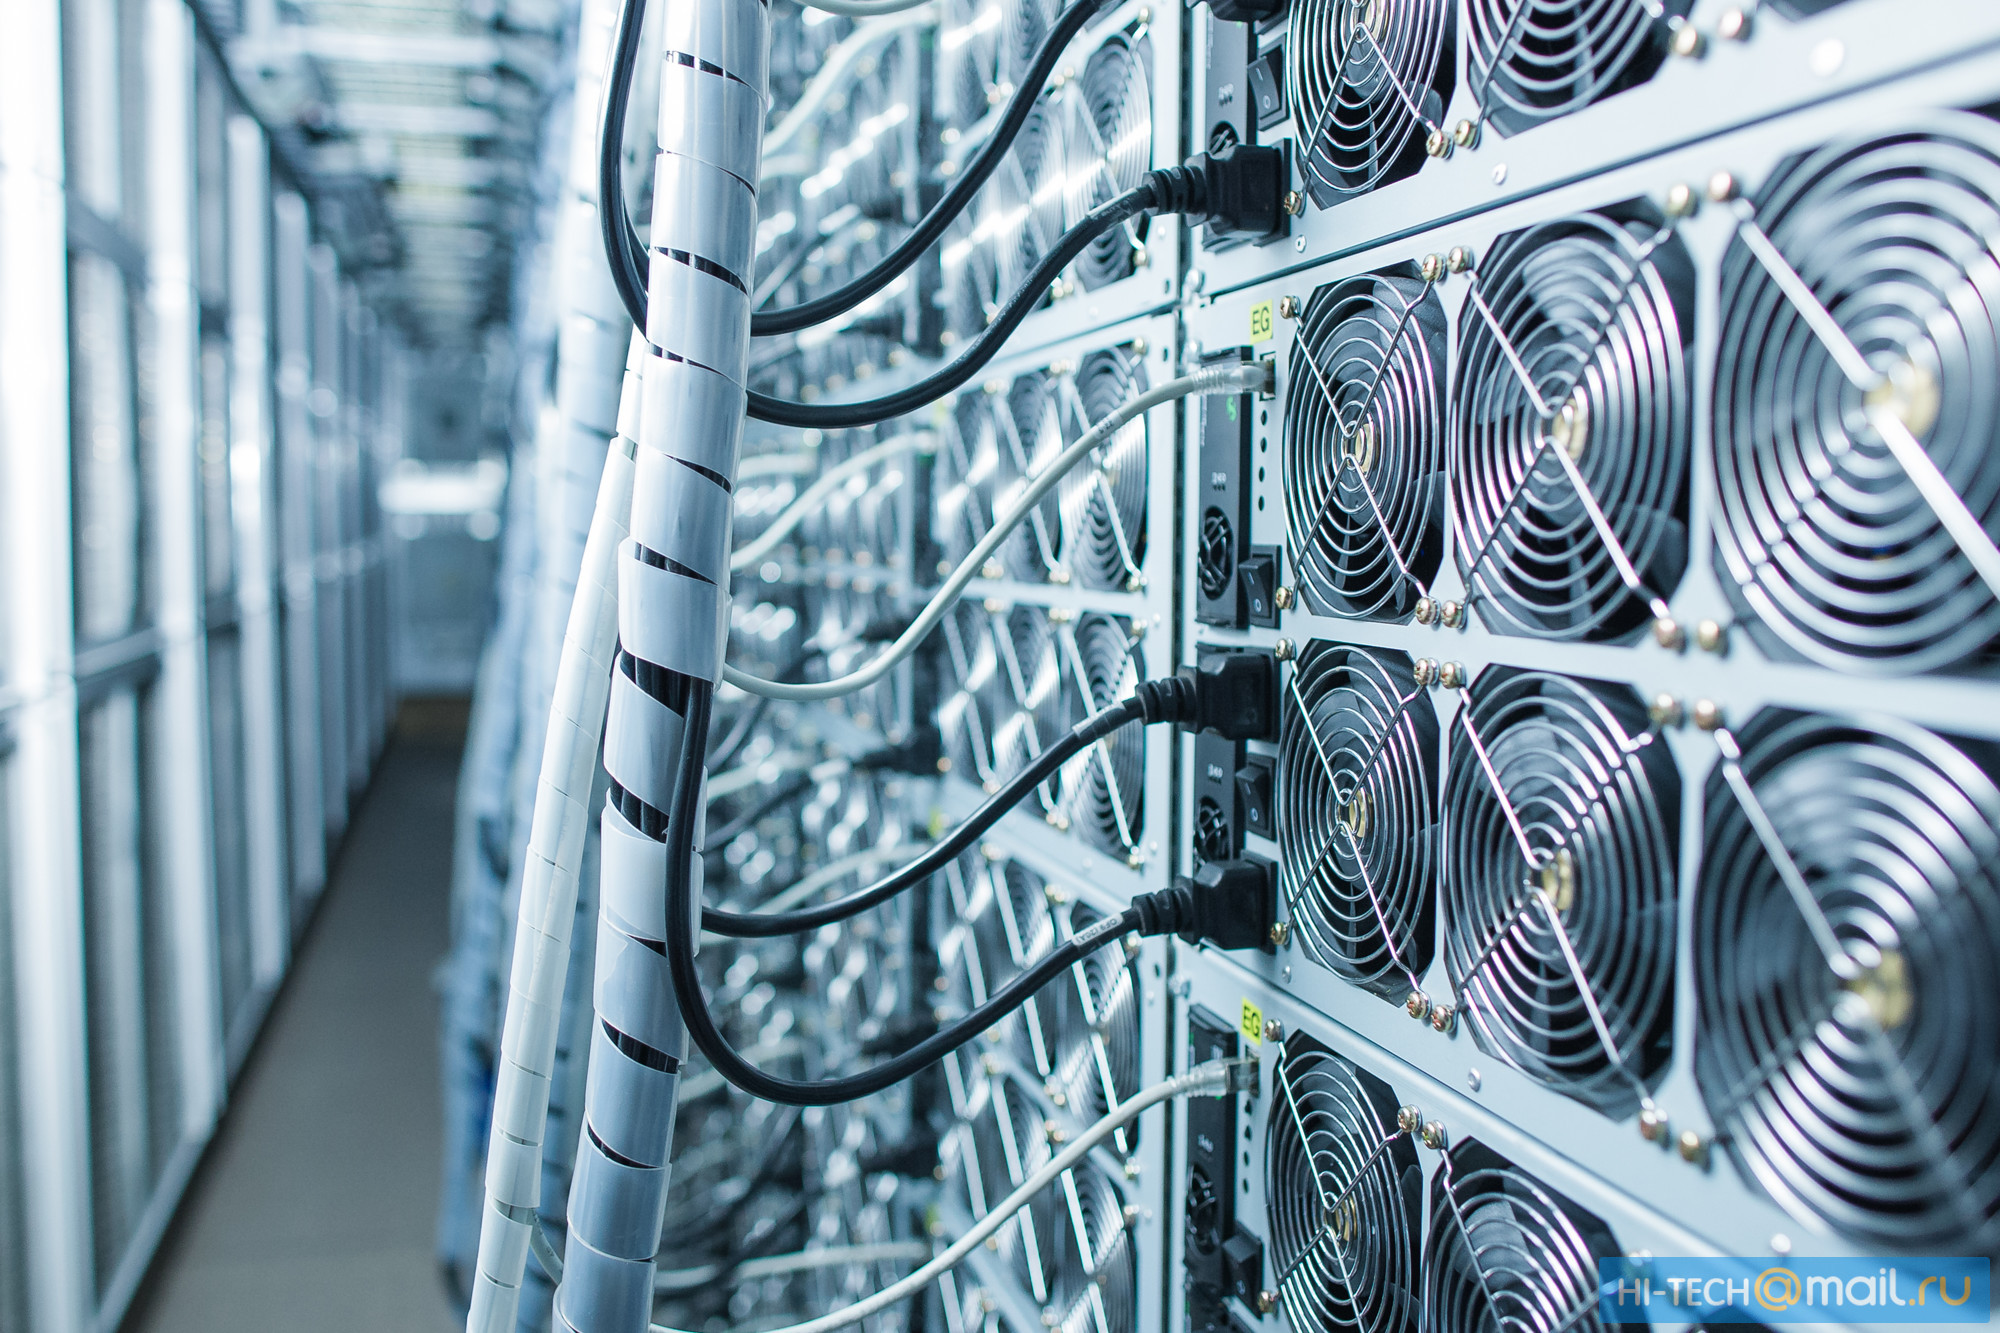
\includegraphics[width=\textwidth]{Images/mining02.jpg}
\caption{\label{fig:mine02}Стойки с майнинг-фермами.}
\end{figure}

\end{frame}

\begin{frame}

\begin{figure}
\center
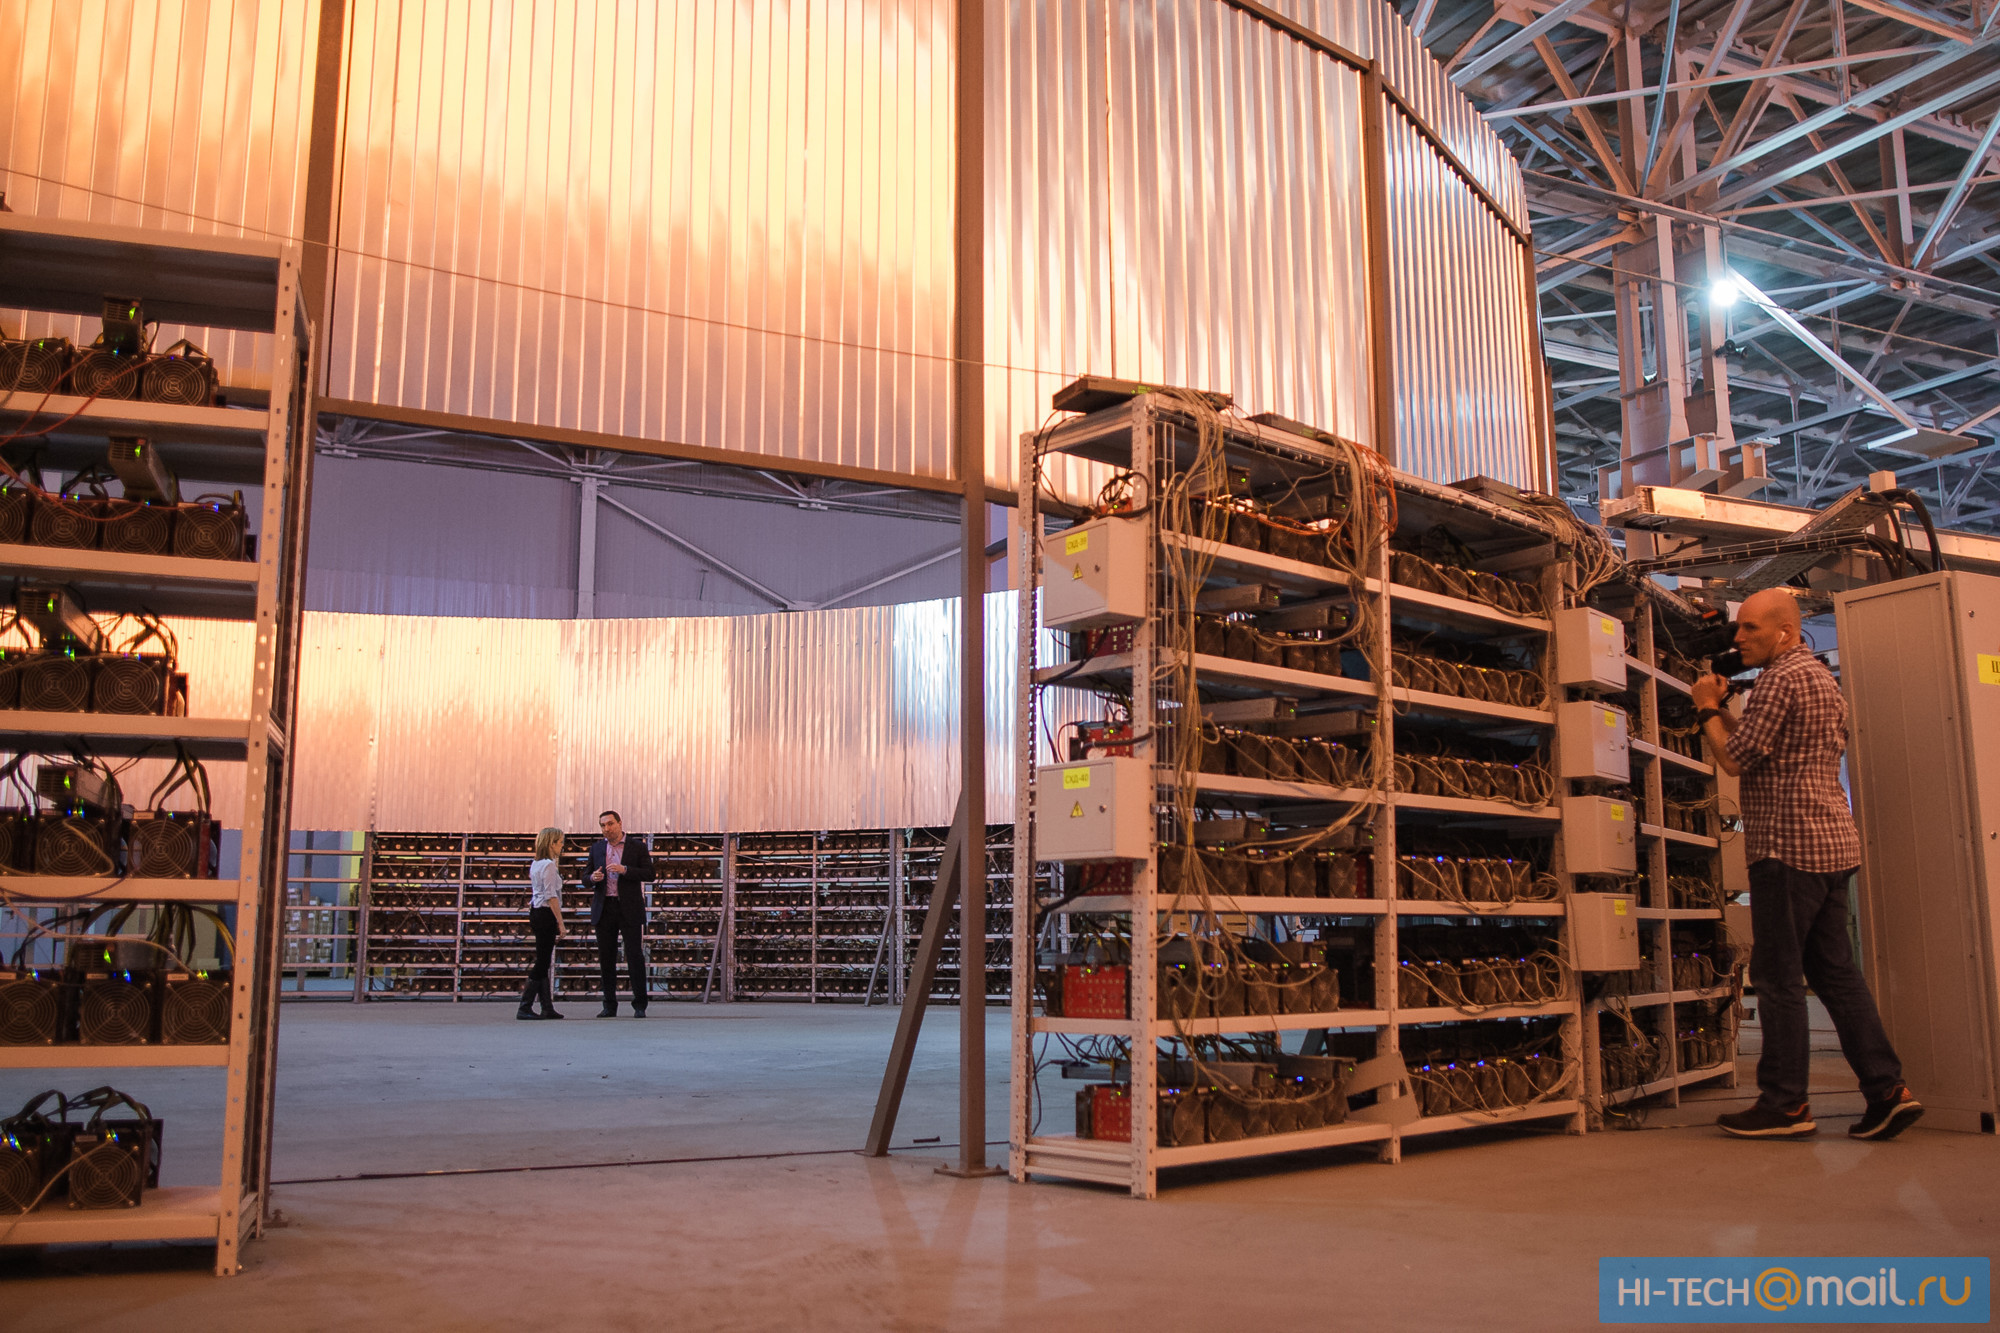
\includegraphics[width=\textwidth]{Images/mining01.jpg}
\caption{\label{fig:mine01}Цех майнинга на заводе <<Москвич>>.}
\end{figure}

\end{frame}


\end{document}
